% ------------------------------------------------------------------------------
% Graduation Project Documentation of Wanas Project ECU Egypt
% ------------------------------------------------------------------------------
\documentclass[11pt]{report} 
\let\cleardoublepage\clearpage

\tracinglostchars=3 % Make it an error if a glyph is missing from the current font
% \cleardoubleoddpage
\usepackage{projectreport}
\usepackage{tikz}
\usetikzlibrary{shapes, arrows, positioning}
% ------------------------------------------------------------------------------

% Enter your details here
% ----------------------------------------------a;sdlkfj--------------------------------
\usepackage{xcolor}  
% \usepackage{Arial}
% \usepackage[T1]{fontenc}
% \usepackage{mathptmx}
\newcommand{\name}{Mahmoud Essam Fathy 191900203\\[6pt]Hader Farag 191900162\\[6pt]Mariem Kamel 191900053\\[6pt]Mohamed Khaled 191900260\\[6pt]Alaa Kamal 191900057\\[6pt]}
\newcommand{\course}{Graduation Project Report}
% \newcommand{\course}{BSc. (Hons) Financial Mathematics}
% \newcommand{\course}{MMath. (Hons) Mathematics}
% \newcommand{\course}{BSc. (Hons) Secondary Mathematics Education with QTS}
\newcommand{\projecttitle}{Wanas}
\newcommand{\submissiondate}{December 2023}
\usepackage{svg}
\usetikzlibrary{shapes.geometric, arrows.meta,automata}
\usepackage{forest}



% ------------------------------------------------------------------------------
% Document
% ------------------------------------------------------------------------------
\begin{document}

% \tikz[remember picture,overlay] \node[opacity=0.3,inner sep=0pt] at (current page.center){\includegraphics[width=\paperwidth,height=\paperheight]{bg}};


    \maketitle

% ------------------------------------------------------------------------------
% Top matter
% ------------------------------------------------------------------------------
\chapter*{Abstract}
This graduation project delves into the realm of mental health support by introducing an innovative application designed to act as a virtual therapist. In a world where the pace of life is relentless and mental well-being is of paramount importance, our project aims to leverage artificial intelligence and machine learning to provide accessible and personalized assistance. The virtual therapist application offers users a confidential and empathetic space to express their thoughts and emotions, fostering a sense of connection and understanding. This documentation explores the design principles, underlying technologies, and ethical considerations that guided the development of the application. Additionally, it delves into the potential impact of such a solution on mental health care, addressing the pressing need for accessible and stigma-free support in today's digital landscape. Join us on this journey as we navigate the intersection of technology and mental health, contributing to the ongoing dialogue about innovative solutions for well-being in the modern age.

\chapter*{Acknowledgements}
We express deep gratitude for the collective support and contributions received during the completion of the graduation project. Special thanks are extended to academic mentors, advisors, peers, friends, family, participants, and the technological community. The acknowledgment emphasizes the collaborative nature of the project, recognizing the guidance, inspiration, and resources provided by various individuals and entities. It concludes with a sincere appreciation for everyone who played a role in the project's success and contributed to the academic and professional growth of the individuals involved.
Wanas team\\
ECU\\
2023
\tableofcontents 
\listoffigures
% \listoftables
% \lstlistoflistings		% comment out if not needed

% ------------------------------------------------------------------------------
% Main matter
% Chapters are added to the document using the \include{chapterx} command
% ------------------------------------------------------------------------------
\newpage
\setcounter{page}{0}
\pagenumbering{arabic}
 ------------------------------------------------------------------------------
% Chapter 1
% ------------------------------------------------------------------------------
\chapter{Introduction} % enter the name of the chapter here
\section{ProjectIdea} % enter the name of the section here
\subsection{why?} %enter the name of the subsection here




 ------------------------------------------------------------------------------
% Chapter 1
% ------------------------------------------------------------------------------
\chapter{Introduction} % enter the name of the chapter here
Mental health is a state of well-being that allows an individual to feel, think and act to their full potential. They are an integral part of health and well-being that underpin our individual and collective abilities to make decisions, establish relationships and shape the world in which we live. Mental health affects every aspect of our lives, including our physical health, our social relationships, our productivity at work or school, and our general sense of well-being. When our mental health is good, we are able to deal with daily challenges and feel happy and satisfied with life. However, mental health is an important issue that is often overlooked. In fact, according to the World Health Organization, about 1 in 4 people in the world will suffer from a mental disorder at some point in their lives. There are many reasons why people hesitate to seek help from psychiatrists. One reason is fear of stigma. There are still a lot of social judgments around mental health, and some people fear they will be seen as weak or unstable if they seek help. Another reason for hesitation is fear of cost. Mental health care can be expensive, especially in low- or middle-income countries. Finally, some people may find it difficult to talk about their feelings and experiences with a psychologist. They may feel ashamed or afraid of being judged. Therefore, we present the WANAS application, through which we provide an innovative solution to these challenges, where individuals can talk to artificial intelligence to obtain support and guidance at any time.
\section{ProjectIdea} % enter the name of the section here
The graduation project centers around the development of an application designed to function as a virtual therapist. The primary goal is to provide accessible and personalized mental health support in an increasingly fast-paced and interconnected world. The application utilizes artificial intelligence and machine learning to create an empathetic and intelligent virtual therapist capable of engaging with users in a meaningful way.

Key Features:

    Personalized Support: The virtual therapist is designed to offer tailored assistance, taking into account individual needs, preferences, and mental health concerns. Through advanced algorithms, the application adapts its responses to the user's specific emotional state and context.

    Confidential and Non-Judgmental Space: Recognizing the importance of privacy in mental health discussions, the application creates a secure and confidential environment. Users can freely express their thoughts and emotions without fear of judgment, fostering a sense of trust and openness.

    User-Friendly Interface: The project prioritizes a user-friendly interface to ensure that individuals, regardless of their technological proficiency, can easily navigate and interact with the virtual therapist. The goal is to make mental health support accessible to a broad audience.

    Integration of AI and Machine Learning: Leveraging the latest advancements in artificial intelligence and machine learning, the virtual therapist continuously learns and improves its responses over time. This dynamic adaptation ensures a more effective and personalized support system for users.

    Addressing Mental Health Stigma: The project aims to contribute to the destigmatization of mental health issues by providing a digital platform that encourages users to seek help in a discreet and comfortable manner.

Throughout the development process, ethical considerations are a key focus, ensuring user privacy, data security, and adherence to established mental health care guidelines. The project envisions making a meaningful impact on the mental well-being of individuals globally by offering a modern, technology-driven approach to mental health support.
 
\subsection{why?} %enter the name of the subsection here
The need for the virtual therapist application arises from several compelling reasons, addressing significant challenges in the current landscape of mental health care:

    Accessibility and Timeliness: Traditional mental health services often face challenges related to accessibility and timely support. The virtual therapist application fills this gap by providing immediate assistance, allowing users to access support whenever they need it, without the constraints of scheduling appointments or geographical limitations.

    Stigma Reduction: Mental health stigma remains a formidable barrier to seeking help. By offering a confidential and non-judgmental space, the application contributes to destigmatizing mental health issues. Users can engage with the virtual therapist discreetly, reducing the fear of social repercussions and promoting a more open dialogue about mental health.

    Global Reach: In a world where mental health issues are pervasive and diverse, a digital solution provides a scalable and globally accessible platform. The virtual therapist application has the potential to reach individuals in remote areas or regions with limited mental health resources, democratizing access to support services.

    Personalization and Adaptability: Every individual's mental health journey is unique, requiring personalized support. The application utilizes artificial intelligence and machine learning to adapt its responses to the specific needs and emotional states of users. This personalized approach enhances the effectiveness of the support provided.

    24/7 Support: Mental health concerns do not adhere to a fixed schedule. The virtual therapist application offers continuous support, 24 hours a day, 7 days a week. This ensures that users can seek assistance at any time, particularly during moments of crisis or when faced with urgent emotional challenges.

    Complementary Support to Traditional Services: The application is designed to complement traditional mental health services rather than replace them. It serves as an additional resource, offering immediate support and guidance, while also encouraging users to seek professional help when necessary.

    Technological Advancements: With the rapid advancement of technology, leveraging artificial intelligence and machine learning in mental health care represents a logical progression. The virtual therapist application harnesses these technologies to enhance the quality and accessibility of mental health support.

In summary, the virtual therapist application is a response to the evolving needs of individuals in a digital age, providing a convenient, stigma-free, and personalized solution to the challenges associated with mental health care. It aims to empower users to take control of their mental well-being by offering support that is accessible, adaptable, and considerate of the diverse nature of mental health experiences.




 
\chapter{ Analysis And Design} 

In this chapter, we outline the project planning process for the development of an AI-powered mental health application. We delineate the functional and non-functional requirements identified through extensive research, and detail the strategies employed to address these requirements.

\section{Functional Requirements}
Functional requirements delineate the specific features and capabilities that our application must possess to meet the needs and expectations of its users.
\subsection{Login and Register}

The application provides a user-friendly interface for new users to register and existing users to sign in.

\paragraph{User Registration}

If a user wants to register, they can do so in one of the following ways:

\begin{itemize}
    \item \textbf{Creating a New Account:} Users can create a new account by providing necessary details such as username, password, email, and other required information. 
    \item \textbf{Signing Up Using Google or Facebook:} Users have the option to sign up using their existing Google or Facebook accounts. This option simplifies the registration process by allowing users to authenticate using their social media credentials.
\end{itemize}

\paragraph{User Login}

Users who already have an account can sign in to the application by:

\begin{itemize}
    \item \textbf{Standard Login:} Entering their registered username and password.
    \item \textbf{Social Media Login:} Logging in through their Google or Facebook accounts, provided they have previously registered using these credentials.
\end{itemize}

\begin{figure}[h]
    \includegraphics[width=\columnwidth]{login}
    \caption{Login and Registration Flow Digram}  
    \centering
    \end{figure}



\subsection{Chat with AI}

The application allows users to initiate and engage in chat sessions with the AI, enabling them to have meaningful conversations and seek mental health support.

\paragraph{Users can :}

\begin{itemize}
    \item \textbf{Starting a New Conversation:} Users can click on the "Start Chat" button to initiate a new conversation with the AI. 
\end{itemize}

\subsection{Persona List}

The Persona List feature allows users to create and manage a list of characters with whom they can engage in conversations. The application saves all interactions with each character, providing a personalized experience.

\paragraph{Users can:}

\begin{itemize}
    \item \textbf{Create New Persona:} Add new personas by providing Persona details such as name.
    \item \textbf{Edit Existing Persona:} Modify details of existing personas to update their characteristics.
    \item \textbf{Delete Persona:} Remove Personas from the list if they are no longer needed.
\end{itemize}



    \subsection{Chat List}

Within each persona, the Chat List feature provides a detailed list of conversations the user has had with that character. This organization helps users manage and review their interactions effectively.

\paragraph{Users can:}

\begin{itemize}
    \item \textbf{Select a Persona:} Choose a persona from the Persona List to view all associated conversations.
    ry in the Chat List includes the date and time of the conversation, providing a chronological overview.
    \item \textbf{Access Detailed Chats:} Click on an entry to view the full conversation, allowing users to revisit and analyze past interactions.
\end{itemize}

\subsection{Previous Conversations}

The application provides a feature for users to view their previous interactions, allowing them to track and reference past conversations with ease.

\paragraph{Users can:}

\begin{itemize}
    \item \textbf{View Details:} Each conversation entry includes the name of the interaction, duration, and date. This provides users with a quick overview of their past chats.
    \item \textbf{Select and Review:} Users can select a conversation to review the chat history, facilitating continuity and reference to past discussions.
\end{itemize}

\subsection{Positive Card}

The application includes an interactive \textit{Positive Card} feature designed to enhance the user's mood and foster positivity.

\paragraph{Functionality of the Positive Card}

The Positive Card provides:

\begin{itemize}
    \item \textbf{Interactive Content:} Engaging content such as motivational quotes, positive affirmations, or uplifting messages tailored to improve the user's mood.

\end{itemize}

\subsection{Mood Tracker}

The Mood Tracker feature allows users to monitor their emotional state over time, helping them identify their emotions in the period of using the app and effectively manage their mental health.

\paragraph{Users can:}

\begin{itemize}
 \item \textbf{Log emotional states:} Record your mood at different times throughout the day or week, or choose from predefined categories.
 \item \textbf{View Mood History:} Access a historical record of your recorded moods, presented in an intuitive interface that includes graphs or charts showing mood trends over time.

\end{itemize}


\section{Non-Functional Requirements}
Non-functional requirements encompass the attributes that characterize the overall performance, usability, and scalability of our application.

\subsection{Security and Privacy}

Ensuring the security and privacy of user data is paramount in our application. We implement robust security measures to maintain the confidentiality of users and ensure complete privacy. Data protection is enforced through secure communication channels and encryption between the server, the user, and the AI model.

\paragraph{Data Protection}

\begin{itemize}
    \item \textbf{Encryption:} All user data is encrypted during transmission and storage to prevent unauthorized access.
    \item \textbf{Secure Authentication:} Implement secure authentication mechanisms such as multi-factor authentication to verify user identity.
    \item \textbf{Compliance:} Adhere to privacy regulations and standards to ensure user data is handled responsibly and legally.
\end{itemize}

\subsection{Speak Comfortably}

Our application supports the Arabic language, enabling users to communicate comfortably and express themselves accurately in their native language. This language support is crucial for effective interaction and user satisfaction.

\subsection{Speed Of Response}

our application is designed to provide rapid responses to user inputs, facilitating a smooth and continuous conversation experience without long wait times.

\subsection{Usability and User Experience}

Our application features a user-friendly interface that is simple and easy to navigate, allowing users to interact with the application effortlessly.

\paragraph{User-Centric Design}

\begin{itemize}
    \item \textbf{Intuitive Interface:} We  Designed an interface that is easy to learn and use, with clear navigation and well-organized elements.
    \item \textbf{Aesthetic Appeal:}we  Ensured the visual design is appealing and enhances the user experience.
 
\end{itemize}



\section{Implementation Strategies}

To address the identified functional and non-functional requirements, various implementation strategies and technologies are employed in the development of the application.

\subsection{Cross-Platform Development with Flutter}

Utilizing Flutter for cross-platform development enables applications to reach a broader audience across different devices and operating systems, enhancing accessibility and user engagement. Flutter’s unique approach to building natively compiled applications for mobile, web, and desktop from a single codebase ensures that the application can cater to a diverse user base without needing separate versions for each platform. This strategy saves significant time and resources \cite{flutter_overview}.

\subsection{Advantages of Flutter} 

\paragraph{Broader Accessibility} Flutter allows the application to be compatible with various operating systems, including iOS, Android, Windows, macOS, Linux, and Web. This wide range of support ensures that users can access the application regardless of their preferred device or platform .

\paragraph{Consistent User Experience} Flutter provides a rich set of customizable widgets and its own rendering engine, enabling the creation of a consistent user experience across different devices. This consistency is crucial for delivering a seamless and unified user interface and interaction flow, which enhances user satisfaction and engagement. The ability to achieve pixel-perfect UI on various platforms ensures that users enjoy a similar experience, irrespective of the device they use \cite{flutter_cons_pros}.

\paragraph{Cost-Efficiency} Flutter’s approach to a single codebase for multiple platforms significantly reduces development costs compared to creating and maintaining separate codebases for each platform. This cost-efficiency extends to updates and maintenance since changes can be implemented once and reflected across all platforms, eliminating the need for redundant development efforts \cite{codecademy_flutter}.

\paragraph{Faster Time-to-Market} Flutter accelerates the deployment process by allowing the development of a single codebase that can be compiled into applications for multiple platforms. This rapid development and deployment capability are crucial for addressing user needs promptly and maintaining competitiveness in the market. Flutter's hot-reload feature further speeds up the development process by enabling real-time changes without restarting the app \cite{flutter_hot_reload}.

\paragraph{Simplified Testing} With a unified codebase in Flutter, the testing process is streamlined, allowing developers to identify and address issues more efficiently. This simplification ensures higher quality and reliability of the application across all supported platforms. Additionally, Flutter’s comprehensive testing framework supports unit, widget, and integration testing, facilitating thorough testing processes \cite{flutter_testing}.



\subsection{programming languages}

The choice of programming languages plays a crucial role in the development of the application. Go is utilized for server-side programming due to its efficiency, concurrency support, and scalability, while Python is leveraged for artificial intelligence programming owing to its extensive libraries and frameworks tailored for machine learning and natural language processing tasks.

\subsection{Server-Side Programming with Go}

\paragraph{Efficiency and Performance:} Go (Golang) offers excellent performance due to its compiled nature and efficient garbage collection. This performance is crucial for handling large volumes of requests and ensuring smooth operation of the application \cite{golang_efficiency}.

\paragraph{Concurrency Support:} Go’s native support for concurrency through goroutines allows the application to manage multiple processes simultaneously, enhancing the system’s ability to handle concurrent user interactions and background tasks \cite{golang_concurrency}.

\paragraph{Scalability:} Go’s design principles and simplicity make it well-suited for building scalable server-side applications, ensuring the AI mental health application can grow and adapt to increasing user demands \cite{golang_scalability}.

\subsection{AI and Machine Learning with Python}

\paragraph{Extensive Libraries:} Python is chosen for artificial intelligence programming due to its rich ecosystem of libraries and frameworks, such as TensorFlow, Keras, and scikit-learn. These tools provide robust support for developing and deploying AI models, including those for natural language processing and sentiment analysis \cite{tensorflow, keras, scikit_learn}.

\paragraph{Ease of Integration:} Python’s flexibility and ease of integration with other technologies facilitate the incorporation of AI capabilities into the application, enabling the development of sophisticated mental health support features \cite{python_integration}.


\section{System analysis through formal diagrams }

The next section provides a detailed analysis of the system through Four formal diagrams and a wireframe. These diagrams will delve into different aspects of the system, including an outline of what the application looks like, users interacting with it (Use Cases), its internal processes (activities), and the flow of communications between components (sequences). In addition, they will identify the basic elements (Class Digram) of the system and its different operational states.

\subsection{Wireframe}
In this wireframe, we present the initial design of the application and present the most important requirements that make up the application

\begin{figure}[h]
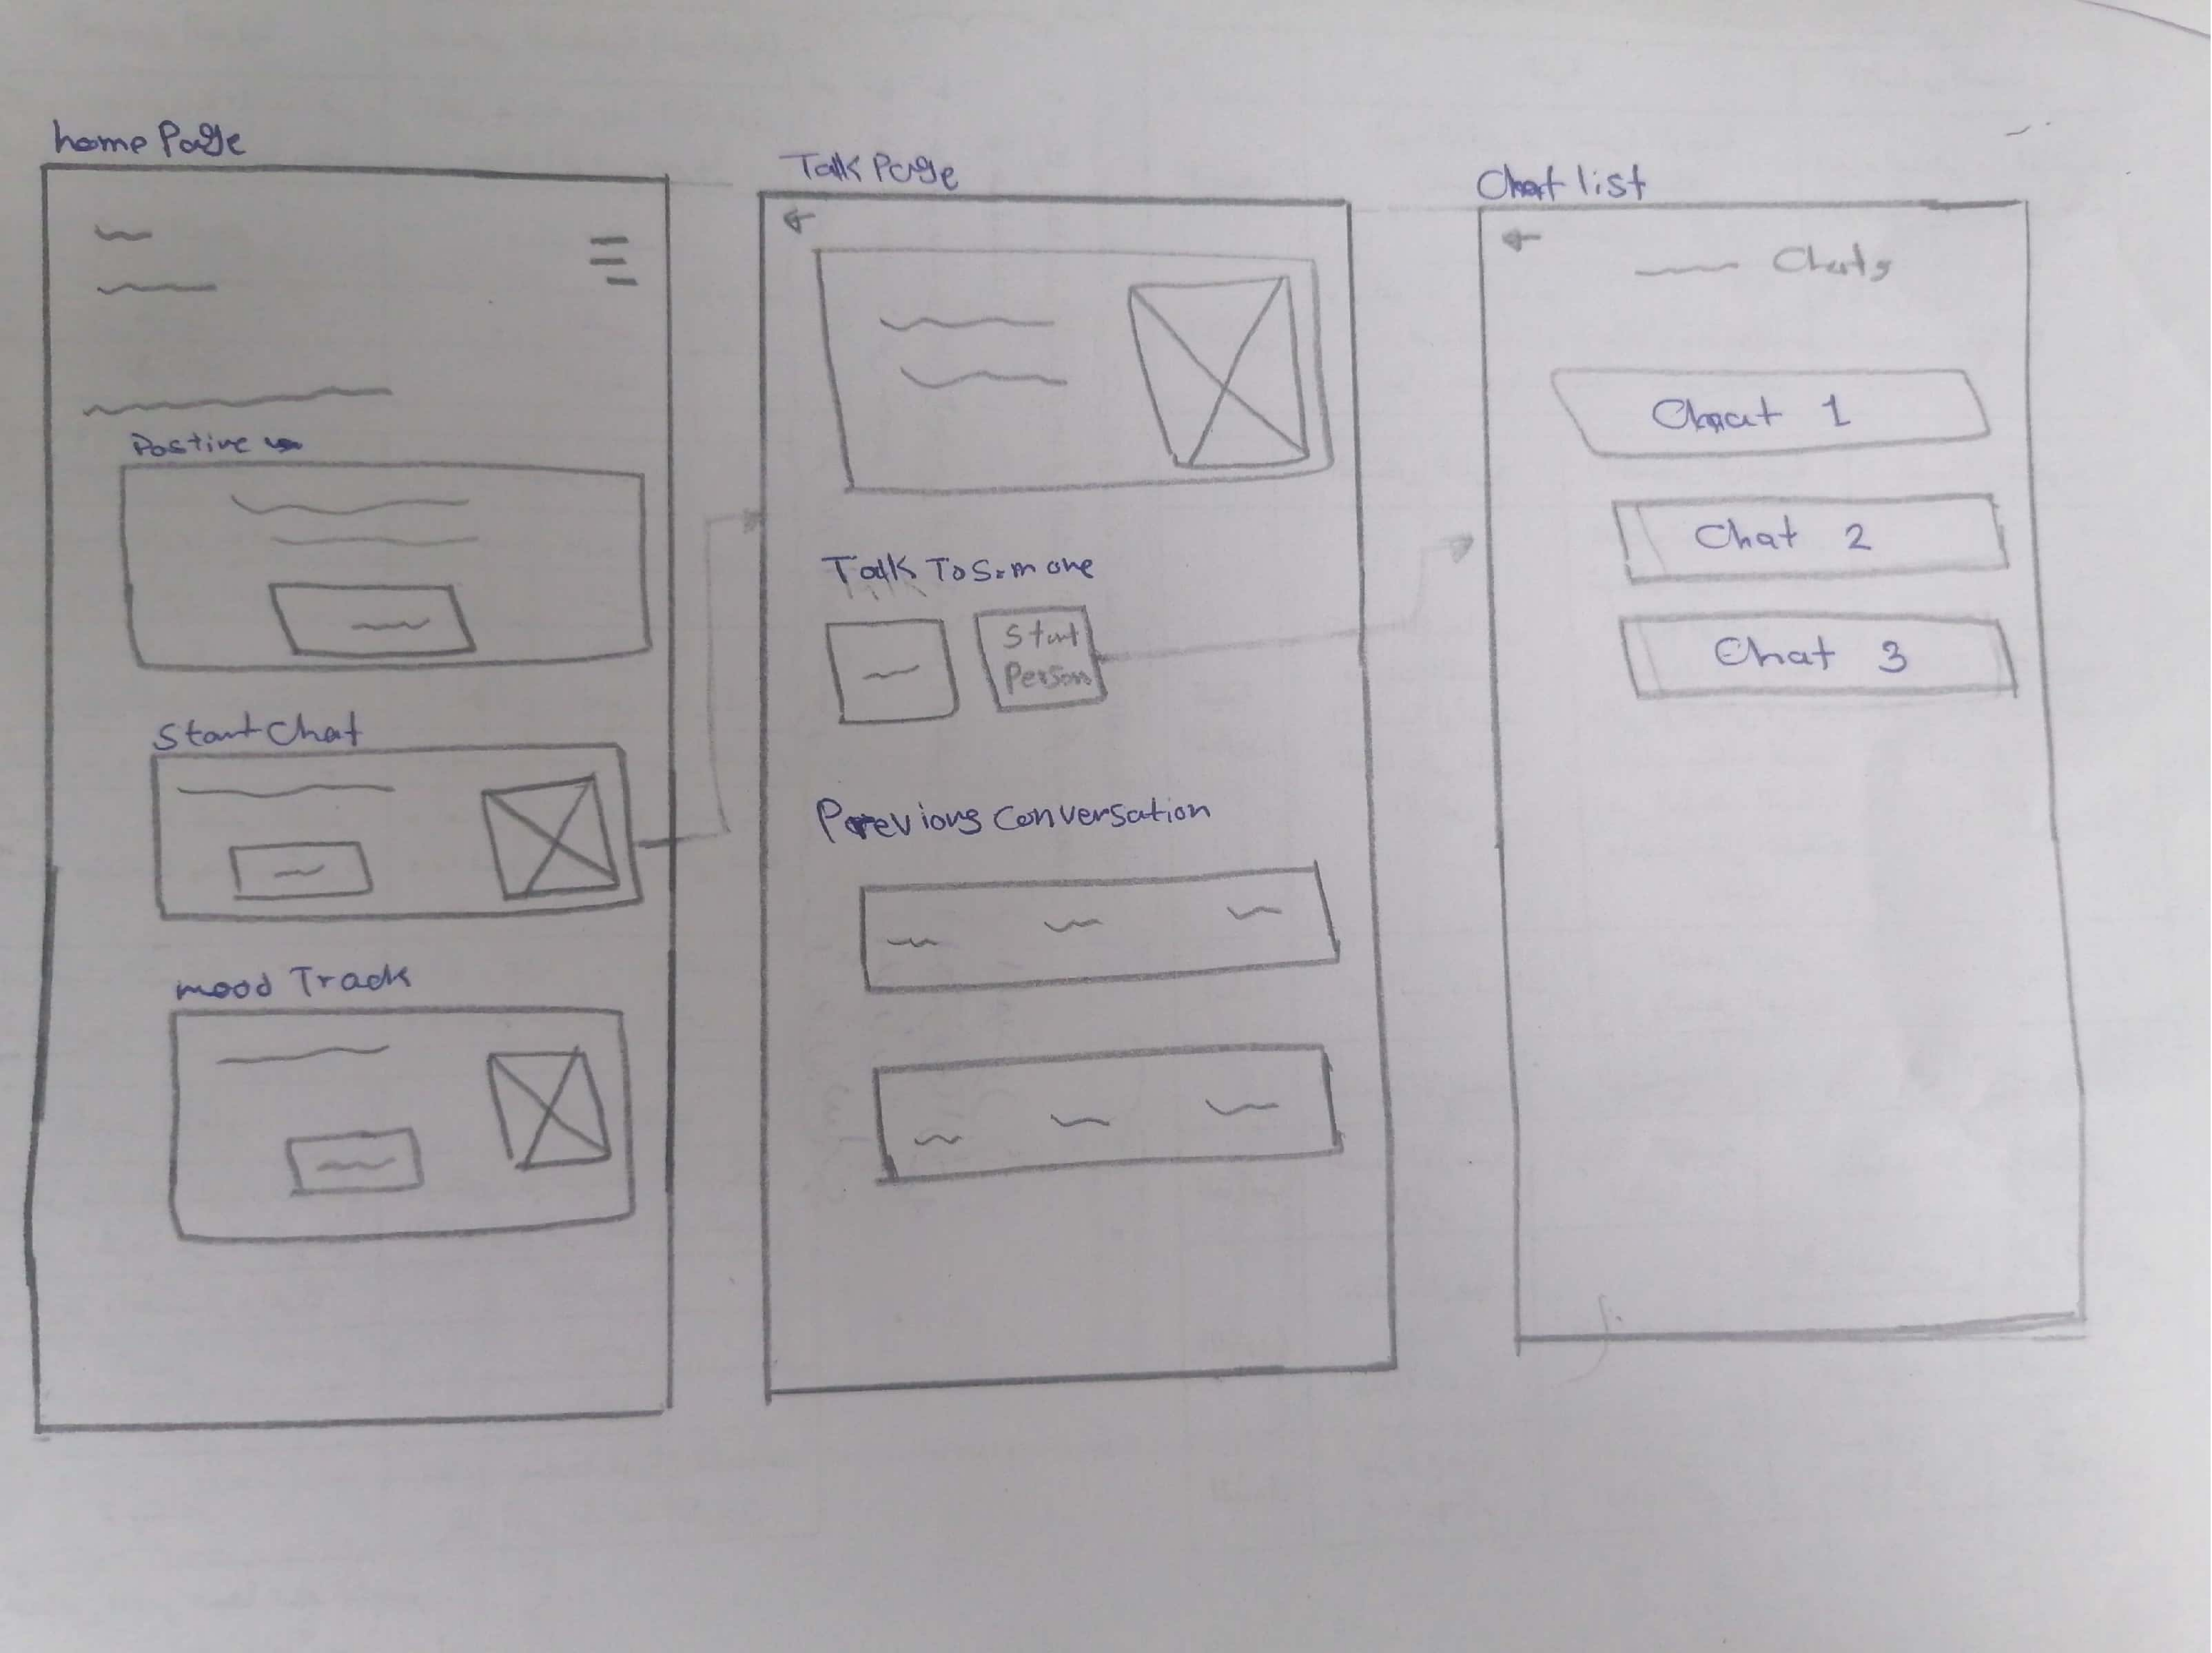
\includegraphics[width=0.5\textwidth, height=0.5\textheight]{wf}
\caption{Wireframe for the main screen of application}
\centering
\end{figure}

\subsection{Use Case Diagram }
The use case diagram depicts an app "WANAS," with the user as the central actor. It outlines the actions users can perform within the system, such as registering, logging in, editing their profiles, starting a chat, interacting with personas, tracking their mood, accessing tips, deleting their account, and logging out. There are also extended use cases, including editing passwords, email, and pictures, suggesting a focus on user management and personalization.

\begin{figure}[h]
    \includegraphics[width=0.8\textwidth, height=0.7\textheight]{fuc}
    \caption{Use Case for application}
    \centering
    \end{figure}

 
    \subsection{Activity Diagram }
    The flow of actions that the user can perform is depicted in the following figure: 
    \begin{itemize}
        \item  It displays the flow of the Login and Register processes. The user can select to reach the home page by registering to create a new account or by logging in if he already has one. Without validating, the user won't be able to view the home page.
        \item  After logging in user can make changes in his profile , start chat , personas list , choose mood.
     
    \end{itemize}
    
    \begin{figure}[h]
        \includegraphics[width=0.8\textwidth, height=0.7\textheight]{acdi}
        \caption{Activity diagram for application}
        \centering
        \end{figure}
    


      \subsection{Sequence Diagram }
      The sequence diagram shows the interactions between a user and a system in a chat application. The user starts by logging in or registering. After successful authentication, the user can create a chat, choose a state, edit the state, edit their profile picture, edit their email, or edit their password. The system interacts with the database to save and retrieve user data and chat information. The mood tracker and the profile features are also represented in the diagram.
    
    
            \begin{figure}[h]
                \includegraphics[width=0.8\textwidth, height=0.7\textheight]{seq}
                \caption{Sequence diagram for application}
                \centering
                \end{figure}
 \subsection{Class Diagram }
 The following figures represents the functions and attributes of the four main classes that the system use :
 \begin{itemize}
 \item  Persona .
 \item  User.
 \item  Message .
 \item  Chatbot.
\end{itemize}
  \begin{figure}[h]
       \includegraphics[width=0.7\textwidth, height=0.5\textheight]{ccd}
     \caption{Class diagram for application}
     \centering
    \end{figure}
          
 
% \include{chapter4} 
 ------------------------------------------------------------------------------
% Chapter 5
% ------------------------------------------------------------------------------
\chapter{AI} % enter the name of the chapter here
\section{Retrieval augmented generation (RAG)} % enter the name of the section here
Retrieval augmented generation (RAG) is a natural language processing (NLP) technique that combines the strengths of both retrieval- and generative-based artificial intelligence (AI) models
\begin{figure}[h]
\includegraphics[width=\columnwidth]{rag}
\centering
\end{figure}
\subsection*{why?}
RAG allows the LLM to present accurate information with source attribution
\subsection{Selecting Documents} %enter the name of the subsection here
First we have select an infromative documents to make the bot therapiest more informative and take the right decision towards the correct and scientific response towards the solution.
so we collected alot of arabic base and translated books and documents from scholar we need to collect alot of information so we made a web scraper to take inputs and search in google scholar and get back the top articles and books in pdf to store them for the next step to use them in the rag system to cover alot of points in the theraptic direction
\subsection{Chunking} 
Dividing a large text corpus into smaller, manageable pieces or segments. Each chunk acts as a standalone unit of information that can be individually indexed and retrieved.
\begin{figure}[h]
\includegraphics[width=\columnwidth]{chunking}
\caption{showing the chunking process and adding the chunks to the query}
\centering
\end{figure}

\section*{Chunking Methods}

We considered several chunking methods for processing our PDF text:

\begin{itemize}
    \item Fixed Size Chunking
    \item Recursive Chunking
    \item Document Specific Chunking
    \item Semantic Chunking
    \item Agentic Chunking
\end{itemize}



\section*{Why Semantic Chunking?}

Semantic chunking offers the following advantages:
\begin{itemize}
    \item Fast
    \item Efficient
    \item Accurate
\end{itemize}
Therefore, we chose semantic chunking over the other methods.

\subsection{Similarity Search} 
Similarity Search is the way of RAG to get the targeted related part of the pdfs or chunks to embed the information that is related to the current input in the prompt and get more accurate informative results
\begin{figure}[h]
\includegraphics[width=\columnwidth]{simisearch}
\caption{showing the chunking process and adding the chunks to the query}
\centering
\end{figure}

\subsection{embedding in the prompt}
And after we retrived the chuncks we embed it in the prompt to be passed to the tokenizer and then to the model after that to get the best accurate result to get the knowledge of the therapist embedded in the tuned model to be your friend therapist



\subsection{Introduction}
To enhance our understanding of emotions in text, we decided to create a classification model that takes a user's input message and predicts the corresponding emotion. This model can be particularly useful in sentiment analysis and mental health monitoring. By accurately detecting emotions, we can improve user interactions and provide more empathetic responses.

\begin{figure}[h]
\includegraphics[width=\columnwidth]{emo1}
\centering
\end{figure}

\subsection{Selecting Dataset}
We chose an Arabic dataset named {arabic-empathetic-conversations} for emotion classification. This dataset consists of conversations where each conversation is labeled with an emotion. The dataset has 36,628 rows and 30 unique emotions, organized into three columns: {emotion}, \textit{context}, and \textit{response}. This rich dataset provides a comprehensive basis for training our emotion detection model.

\subsection{Preprocessing}
To prepare the dataset for training, we performed several preprocessing steps:

\begin{figure}[h]
\includegraphics[width=\columnwidth]{emo2}
\centering
\end{figure}
\begin{enumerate}
    \item \textbf{Emotion Selection}: We selected a subset of unique emotions, reducing the dataset size to 5,820 rows. This step helps to focus on the most relevant emotions and reduces the complexity of the model.
    \item \textbf{Combining Text}: We concatenated the {context} and {response} columns into a single column named \textit{text} to represent the entire conversation. This ensures that the model has all the necessary information in a single input field.
    \item \textbf{Label Encoding}: We converted the emotion labels into numerical indices using a mapping dictionary ({lbl2idx}). For example, the mapping looked like this: \{‘joyful’: 0, ‘sad’: 1, ‘lonely’: 2, ‘anxious’: 3, ‘content’: 4\}. This numerical encoding is essential for training machine learning models.
    \item \textbf{Imbalancing}: To address class imbalance, we used the {oversample\_data} function. This function oversamples the minority classes by randomly duplicating samples until each class has the same number of samples as the majority class. This helps prevent the model from being biased towards the majority class during training. The function utilizes the {resample} function from the \textit{sklearn.utils} module.
\end{enumerate}

\section{Data Splitting}
We split the dataset into training, validation, and test sets as follows:

\begin{figure}[h]
\includegraphics[width=\columnwidth]{emo3}
\centering
\end{figure}
\begin{enumerate}
    \item \textbf{Initial Split}: We divided the dataset into training (70\%) and temporary data (30\%) to ensure that the model has enough data to learn from while reserving a portion for testing.
    \item \textbf{Second Split}: We split the temporary data into equal parts for testing and validation (50\% each) to fine-tune the model and evaluate its performance.
\end{enumerate}

The final split sizes were:
\begin{itemize}
    \item Training: 4,074 rows
    \item Validation: 873 rows
    \item Testing: 873 rows
\end{itemize}

This splitting strategy ensures that the model is tested on unseen data, providing a realistic measure of its performance.

\section{Selecting Model}
We chose the BERT model for our classification task, specifically the {aubmindlab/bert-base-arabertv02-twitter} model. BERT (Bidirectional Encoder Representations from Transformers) models are known for their effectiveness in various NLP tasks, including text classification. BERT's ability to understand context from both directions in a sentence makes it particularly powerful for understanding nuanced emotions.

\section{Fine-Tuning}
\begin{enumerate}
    \item \textbf{Model Loading}: We used the {AutoModelForSequenceClassification} class from Huggingface, which helps in loading pre-trained models suitable for sequence classification tasks. We specified the number of labels in our dataset during this step. This class automatically adds a classification head to the model, making it ready for our task.
    \item \textbf{Tokenization}: We used the BERT tokenizer to process the text data. This involved trimming the text to a certain length and adding padding where necessary to ensure uniform input sizes. We also created a custom dataset class to store the tokenized texts and their labels, streamlining the data loading process for training.
\end{enumerate}

\section{Training}
During the training phase, we fine-tuned the BERT model on our preprocessed dataset.
\begin{enumerate}
    \item \textbf{Training Arguments}: We defined various training arguments. These arguments specify where to save the results, how many times to go through the training data, and the number of samples to use in each batch during training and evaluation. They also determine how to adjust the learning rate at the beginning and the strength of weight decay to avoid overfitting. Additionally, the arguments define how often to log and evaluate the model, which in this case is once every epoch.
    \item \textbf{Trainer Class}: We specified the model to be trained in our trainer class and provided the training arguments defined earlier. It also includes the datasets for training and evaluation and a function to calculate performance metrics. This configuration ensures that the model is trained and evaluated with the specified settings, allowing for a structured and efficient training process.
\end{enumerate}

\section{Result}
After fine-tuning the model on our dataset, we evaluated its performance using the validation and test sets. The results demonstrated the model's ability to accurately classify the emotions associated with the given text inputs. Key performance metrics such as accuracy, precision, recall, and F1-score were used to assess the model's effectiveness.

By following these steps, we successfully developed an emotion classification model that can predict emotions from Arabic text inputs. This model can be further refined and applied to various practical applications to understand and respond to human emotions more effectively. Future work could include expanding the dataset, incorporating additional features, and exploring other advanced models to further enhance performance.

\section{LoRA and Q-LoRA}

\section{LoRA}
LoRA (Low-Rank Adaptation) is a technique to fine-tune large language models efficiently by injecting trainable low-rank matrices into each layer of the transformer architecture. This approach reduces the number of parameters that need to be updated during training, making it computationally efficient and cost-effective, especially for tasks requiring adaptation to specific domains or languages.

\section{Q-LoRA}
QLoRA (Quantized Low-Rank Adaptation) builds on LoRA by incorporating quantization techniques. Quantization involves representing model parameters with fewer bits, reducing memory and computational requirements. This saves memory and makes the model run faster, especially on devices with less power.

\begin{figure}[h]
\includegraphics[width=\columnwidth]{emo4}
\centering
\end{figure}
\section{GPU Usage}

\section{Without Q-LoRA}
When we train our model on a GPU without using QLoRA, we use the full precision of the model's parameters.
\begin{enumerate}
    \item \textbf{Full Precision Training}: The model uses 16-bit or 32-bit floating point numbers to represent its parameters. This provides high accuracy but requires more memory and computational power.
    \item \textbf{Memory Usage}: Full precision training uses a lot of GPU memory. For large models, this can quickly fill up the available memory, limiting the batch size and the number of layers we can train simultaneously.
    \item \textbf{Speed}: Training is fast compared to a CPU, but the high memory usage can sometimes slow down the training process if the GPU memory becomes a bottleneck.
    \item \textbf{Results}: Full precision training can lead to slightly better results because there’s no loss of detail in the model’s parameters. However, the difference might not be significant enough to justify the extra resource use.
\end{enumerate}

\section{With Q-LoRA}
When we use QLoRA (Quantized Low-Rank Adaptation) on a GPU, we optimize the training process by reducing the precision of the model’s parameters.
\begin{enumerate}
    \item \textbf{Quantization}: We use 4-bit quantization for the model’s parameters. This means we represent each parameter with fewer bits, drastically reducing the memory footprint.
    \item \textbf{Memory Usage}: With 4-bit quantization, the memory usage drops significantly. This allows us to train larger models or use larger batch sizes without running into memory limitations.
    \item \textbf{Speed}: Training becomes faster because the model is smaller and requires fewer computations. The GPU can process more data in parallel, leading to quicker training times.
    \item \textbf{Results}: While there’s a slight reduction in precision, QLoRA is designed to maintain high performance. The trade-off between memory efficiency and model accuracy is minimal, and in many cases, the results are comparable to full precision training.
\end{enumerate}

\section{Simple Example}
Training a large language model on a GPU without QLoRA might take 10 hours and use up 90\% of the GPU's memory, while training the same model on a GPU with QLoRA might take only 6 hours and use just 50\% of the GPU's memory.

\section{Training Process}
When we train the model, we follow these steps:
\begin{enumerate}
    \item \textbf{Set Up Quantization}: We configure the model to use 4-bit quantization. This reduces the amount of memory the model uses.
    \item \textbf{Prepare the Model}: We prepare the model for training with LoRA. This involves setting up specific parts of the model to be updated.
    \item \textbf{Define LoRA Config}: We define the settings for LoRA, like how many new parameters to add and where to add them in the model.
\end{enumerate}

\section{Detail on Each Step}
\begin{enumerate}
    \item \textbf{Quantization Configuration}: We use a configuration to tell the model to use 4-bit numbers. This helps make the model smaller and faster.
    \item \textbf{Prepare for k-bit Training}: We make the model ready for training with fewer bits. This step involves setting up the model’s layers.
    \item \textbf{LoRA Configuration}: We set parameters like \( r=128 \) and {lora\_alpha=32}. These numbers control how much change we allow in the model. We also specify which parts of the model to update (q\_proj, k\_proj, v\_proj, o\_proj).
\end{enumerate}

\section{Dataset}

\section{Introduction}
We collected our dataset with the help of GPT (AI engine). The dataset consists of raw text conversations on various topics between therapists and their patients. Our goal was to make the dataset as diverse as possible to capture a wide range of interactions.



\section{Emotion Classification Model For Emotion Detection}

\subsection{Preprocessing}
To make the dataset useful for our model, we went through several preprocessing steps:

\subsection{Text Separation}
Each conversation was separated by line. Then splits the conversations using this line.

% \subsection{Data Structuring}
% We created a list where each conversation is represented with a conversation ID and the role (doctor or patient). This list was then saved as a DataFrame with three columns: {['convid', 'role', 'context']}, and totaling 630 rows.
%
\subsection{Detailed Processing}
We initialized an empty list called {final} to store processed chat data and a string {history} to track the conversation history. We looped through each row in the DataFrame:
\begin{itemize}
    \item Added the role and message content to the {history}.
    \item Identified the position in the chat:
    \begin{itemize}
        \item \textbf{First Chat}: Marked as the beginning if it's the first row and the role is "doctor" (doctor).
        \item \textbf{Last Chat}: Marked as the end for the last row:
        \begin{itemize}
            \item For doctors, recorded the conversation with the previous context.
            \item For patients, marked it with "end" (closure).
        \end{itemize}
        \item \textbf{Middle Chats}: Checked if the conversation ID changed:
        \begin{itemize}
            \item Marked as the beginning if a new conversation started.
            \item Marked as the end if a conversation ended.
            \item Recorded patient messages with the previous context for regular chats.
        \end{itemize}
    \end{itemize}
\end{itemize}

\subsection{New DataFrame Creation}
Converted the {final} list into a new DataFrame {dff} with columns: \textit{['history', 'patient', 'doctor']}.

\subsection{Saving and Loading the Dataset}
We saved our dataset as a CSV file. Loaded it from the datasets library on Hugging Face. Used {train\_test\_split} to split the data into training and validation sets with a test size of 0.2.

\section{Why Choosing GPT?}
Choosing the right model is critical for any machine learning project. For a conversational AI like a therapy chatbot, it's important to select a model that understands and generates natural language proficiently and can be fine-tuned to specific conversation contexts.

\section{Model Selection}
We chose to use GPT (Generative Pre-trained Transformer) for our therapy chatbot because of its strong capabilities in understanding and generating natural language. In our model, we decided to choose AceGPT due to its capabilities in understanding and generating Arabic text, which is essential for our application targeting Egyptian Arabic conversations between therapists and patients.

\subsection{First Try: AceGPT7B}
Firstly, we were confused between choosing acegpt7B and acegpt13B, but because we found the differences in sizes between them were small, we decided to choose acegpt13B due to its big training which is on 13 Billion parameters so it’s better to understand our task. In the first try in training this model, it gave us little good answers but it still couldn't chat so well.

\subsection{Second Try: AceGPT13B-Chat}
When using acegpt13Bchat, we noted that the model is too huge and trained on big conversations datasets, so it’s not affected with our tuning by Egyptian friend therapist conversations. So we decided to increase the dataset.

\section{Final Model Choice}
Despite initial challenges with limited data and epochs, integrating LoRA and QLoRA has optimized the model's training process. We successfully enhanced the performance of our model to understand and generate Arabic text effectively.
 
% \include{chapter6} 
% \include{chapter7} 
% ------------------------------------------------------------------------------
% Reference list
% ------------------------------------------------------------------------------

% Specify the bibliography style
% \bibliographystyle{numeric}
\begingroup
\raggedright
\addcontentsline{toc}{chapter}{References}
    \renewcommand\bibname{References}
\printbibliography
\endgroup
% ------------------------------------------------------------------------------
% Appendices
% ------------------------------------------------------------------------------



\include{appendix}

\end{document}

